\documentclass{article}
\usepackage[T1]{fontenc}
\usepackage[utf8]{inputenc}
\usepackage[section]{placeins}
\usepackage{fullpage}
\usepackage{graphicx}
\usepackage{caption}
\usepackage{subcaption}
\usepackage{hyperref}
\usepackage{pgfplots}
\pgfplotsset{compat=1.8}

\hypersetup{colorlinks=true,
			urlcolor=blue,
			linktoc=all,
			linkcolor=black,
			citecolor=black}

\graphicspath{ {./images/} }

\title{CS 4516 Group \#5: Bandwidth Trunking Using Layer 2 Devices\\Results}
\author{Jason Rosenman \and Louis Fogel \and Sam Abradi}
\date{}

\begin{document}
\maketitle
  We collected performance metrics on networks utilizing our switching approach to measure its effectiveness.
  We also measured the performance of an unmodified software switch to allow direct comparison between approaches without encountering issues with    sources of error that may have been introduced by our simulation.
  Due to the fact that neither switch will be implemented in hardware, our performance results may be slightly different because hardware allows for greater parallelism.
  We measured the performance of the network when a link is at saturation to determine the benefit that a redundant bandwidth-sharing link is able to provide.
  We also measured and compared at the goodput of the network in these situations with and without congestion control to show the actual practical effect of our device on end hosts in the network.

\section{Broadcast Storm Mitigation}
\begin{figure}[ht]
	\centering
	\begin{subfigure}[b]{0.4\textwidth}
		\centering
		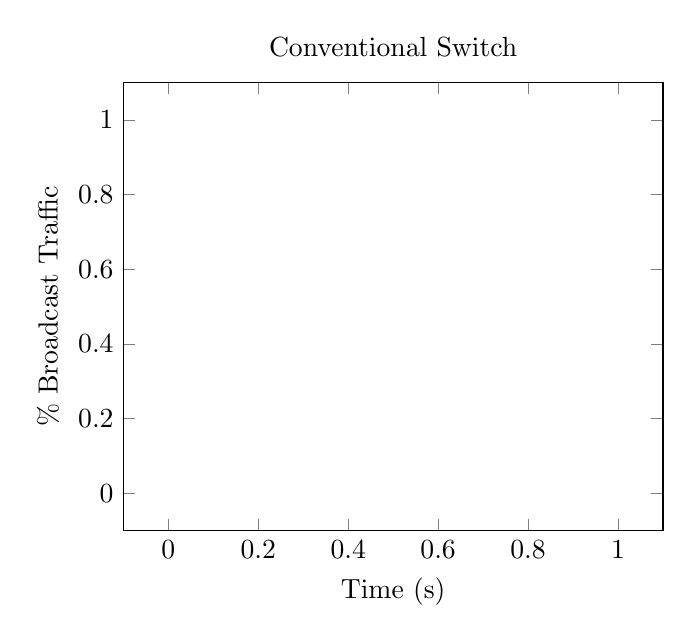
\begin{tikzpicture}
		\begin{axis} [
			title=Conventional Switch,
			xlabel=Time (s),
			ylabel=\% Broadcast Traffic,
		]
% 		\addplot[blue] table {}
		\end{axis}
		\end{tikzpicture}
		\caption{}
		\label{fig:stdbcast}
	\end{subfigure}
	\hfill
	\begin{subfigure}[b]{0.4\textwidth}
		\centering
		\begin{tikzpicture}
		\begin{axis} [
			title=Smart Switch,
			xlabel=Time (s),
			ylabel=\% Broadcast Traffic,
		]
% 		\addplot[blue] table {}
		\end{axis}
		\end{tikzpicture}
		\caption{}
		\label{fig:smtbcast}
	\end{subfigure}
	\caption{Percentage of Broadcast Traffic}
	\label{fig:bcast}
\end{figure}

  To show the effect of broadcast storms on network traffic, we determined the percentage of broadcast frames from total network traffic both with and without a forwarding loop.
  Normally (in a star network with conventional switches), nearly all of the traffic will start as broadcast traffic during the auto-configuration period.
  The amount of broadcast traffic will then drop down to a noise-floor level.
  If the network has a loop in it, the amount of broadcast traffic will not drop off significantly because the network will start a broadcast storm as a result of the forwarding loop.
  Our device exhibits the same drop-off behavior even in a graph network because it filters broadcast packets out of forwarding loops, preventing a broadcast storm from occurring.

\begin{table}[ht]
	\centering
	\caption{Forwarding Loop Goodput}
	\label{tab:goodput}
	% TODO: Add more rows to table for with and without congestion control. Have switch headers span rows.
	\begin{tabular}{|c|c|c|}
		\hline
		& Without Loop	& With Loop \\
		\hline
		Conventional Switch	&	& \\
		\hline
		Smart Switch				&	& \\
		\hline
	\end{tabular}
\end{table}

  Preventing broadcast storms has a noticeable effect on the performance of the network from the perspective of end hosts.
  The average goodput of the network when a forwarding loop exists in the network is significantly improved by our device because it prevents the broadcast storm from occurring.
  These findings are not terribly surprising, but do confirm that the device is capable of preventing broadcast storms without having to disable links.
  This ability is key to the more novel features of the device, bandwidth sharing and seamless fail-over.

\section{Congestion Conditions}
  Situations links in the network are at saturation show the most significant difference in performance between architectures.
  Setups with redundant links perform much better than any other system when there is one flow causing all or most of the congestion, because all of  the other traffic defaults to the other link.
  Single links are unable to provide this service, and as a result they provide markedly worse performance in congestion conditions.
\begin{figure}[ht]
	\centering
	\begin{subfigure}[b]{0.4\textwidth}
		\centering
		\begin{tikzpicture}
		\begin{axis} [
			title=Conventional Switch,
			xlabel=Time (s),
			ylabel=Packet Loss (\%),
		]
% 		\addplot[blue] table {}
		\end{axis}
		\end{tikzpicture}
		\caption{}
		\label{fig:stdbcast}
	\end{subfigure}
	\hfill
	\begin{subfigure}[b]{0.4\textwidth}
		\centering
		\begin{tikzpicture}
		\begin{axis} [
			title=Smart Switch,
			xlabel=Time (s),
			ylabel=Packet Loss (\%),
		]
% 		\addplot[blue] table {}
		\end{axis}
		\end{tikzpicture}
		\caption{}
		\label{fig:smtbcast}
	\end{subfigure}
	\caption{Packet Loss}
	\label{fig:bcast}
\end{figure}
\section{Congestion Control}
  We do not yet know what will happen in this situation.
  The results will come from having hosts send traffic to each other with the default TCP congestion control mechanism in Linux 3.12.9.
  Testing with congestion control may expose flaws in our bandwidth sharing technique, because links only hover near saturation, so the switch may have a hard time determining that more flows need to be moved over to the other link, because the flows will be too interdependent.

\section{Response Time}
  Although our device does require additional processing of broadcast frames, non-broadcast frames can be handled without much additional overhead because they can be quickly found in the flow table.
  Results of our testing indicate that the average response time is not significantly affected by the addition of intelligent switching hardware.
  The advantages of using our device are not offset by any increase in response time from processing, except initially when the flow table is being constructed and when legitimate broadcast traffic is much higher than normal.
\begin{figure}[ht]
	\centering
	\begin{subfigure}[b]{0.4\textwidth}
		\centering
		\begin{tikzpicture}
		\begin{axis} [
			title=Conventional Switch,
			xlabel=Time (s),
			ylabel=Response Time (ms),
		]
% 		\addplot[blue] table {}
		\end{axis}
		\end{tikzpicture}
		\caption{}
		\label{fig:stdbcast}
	\end{subfigure}
	\hfill
	\begin{subfigure}[b]{0.4\textwidth}
		\centering
		\begin{tikzpicture}
		\begin{axis} [
			title=Smart Switch,
			xlabel=Time (s),
			ylabel=Response Time (ms),
		]
% 		\addplot[blue] table {}
		\end{axis}
		\end{tikzpicture}
		\caption{}
		\label{fig:smtbcast}
	\end{subfigure}
	\caption{Response Time}
	\label{fig:bcast}
\end{figure}
\end{document}
